The in-board microcontroller MSP430F5529 (see \autoref{sec:MCU}) executes multiple tasks in parallel. It can:
\begin{itemize}
    \item Enable or disable the power-supplies. 
    \item Monitor the status of the system by activating LEDs on the PCB. 
    \item Modify the gain of the PGA.
    \item Modify the phase of the quadrature-generator. 
    \item Modify the frequency of the square input voltage by programming the Si5351 IC. 
    \item Sample the real and imaginary components of the two electrode pairs current reponse $\Re(V_{PSD-\omega_0}$ and $\Im(V_{PSD-\omega_0}$ at high frequency. 
    \item Sample the voltage of the 5V $V_{DD}$ power-supply at high frequency, and the voltage of the battery at low-frequency. 
    \item Transfer the sampled data to a nearby computer with the help of a FT232RL IC. 
\end{itemize}

It is possible to modify on the fly some of the properties or behavior of the impedance-sensing system. Different commands can be transmitted to the MCU to modify the properties. These commands are shown in \autoref{fig:LoopFlowchart}. \par

The system can be operated in single or multi-frequency modes. The single frequency-mode samples data at a single input frequency. The multi-frequency mode modifies the excitation frequency from an initial frequency up to a maximum frequency each time the sample buffer is full, then it cycles back to the minimum frequency. This technique can be used to obtain the impedance spectroscopy (see \autoref{sec:EIS}) of the SUT. The data transfer can be paused or not. A low-power mode can toggle on if the system is unused for a period of time. Finally, the sampling rate of the system can be toggled between a low constant sampling frequency of 655Hz, and a variable rate high-speed sampling frequency of 5461Hz. \par
\begin{figure}[h]
    \centering
    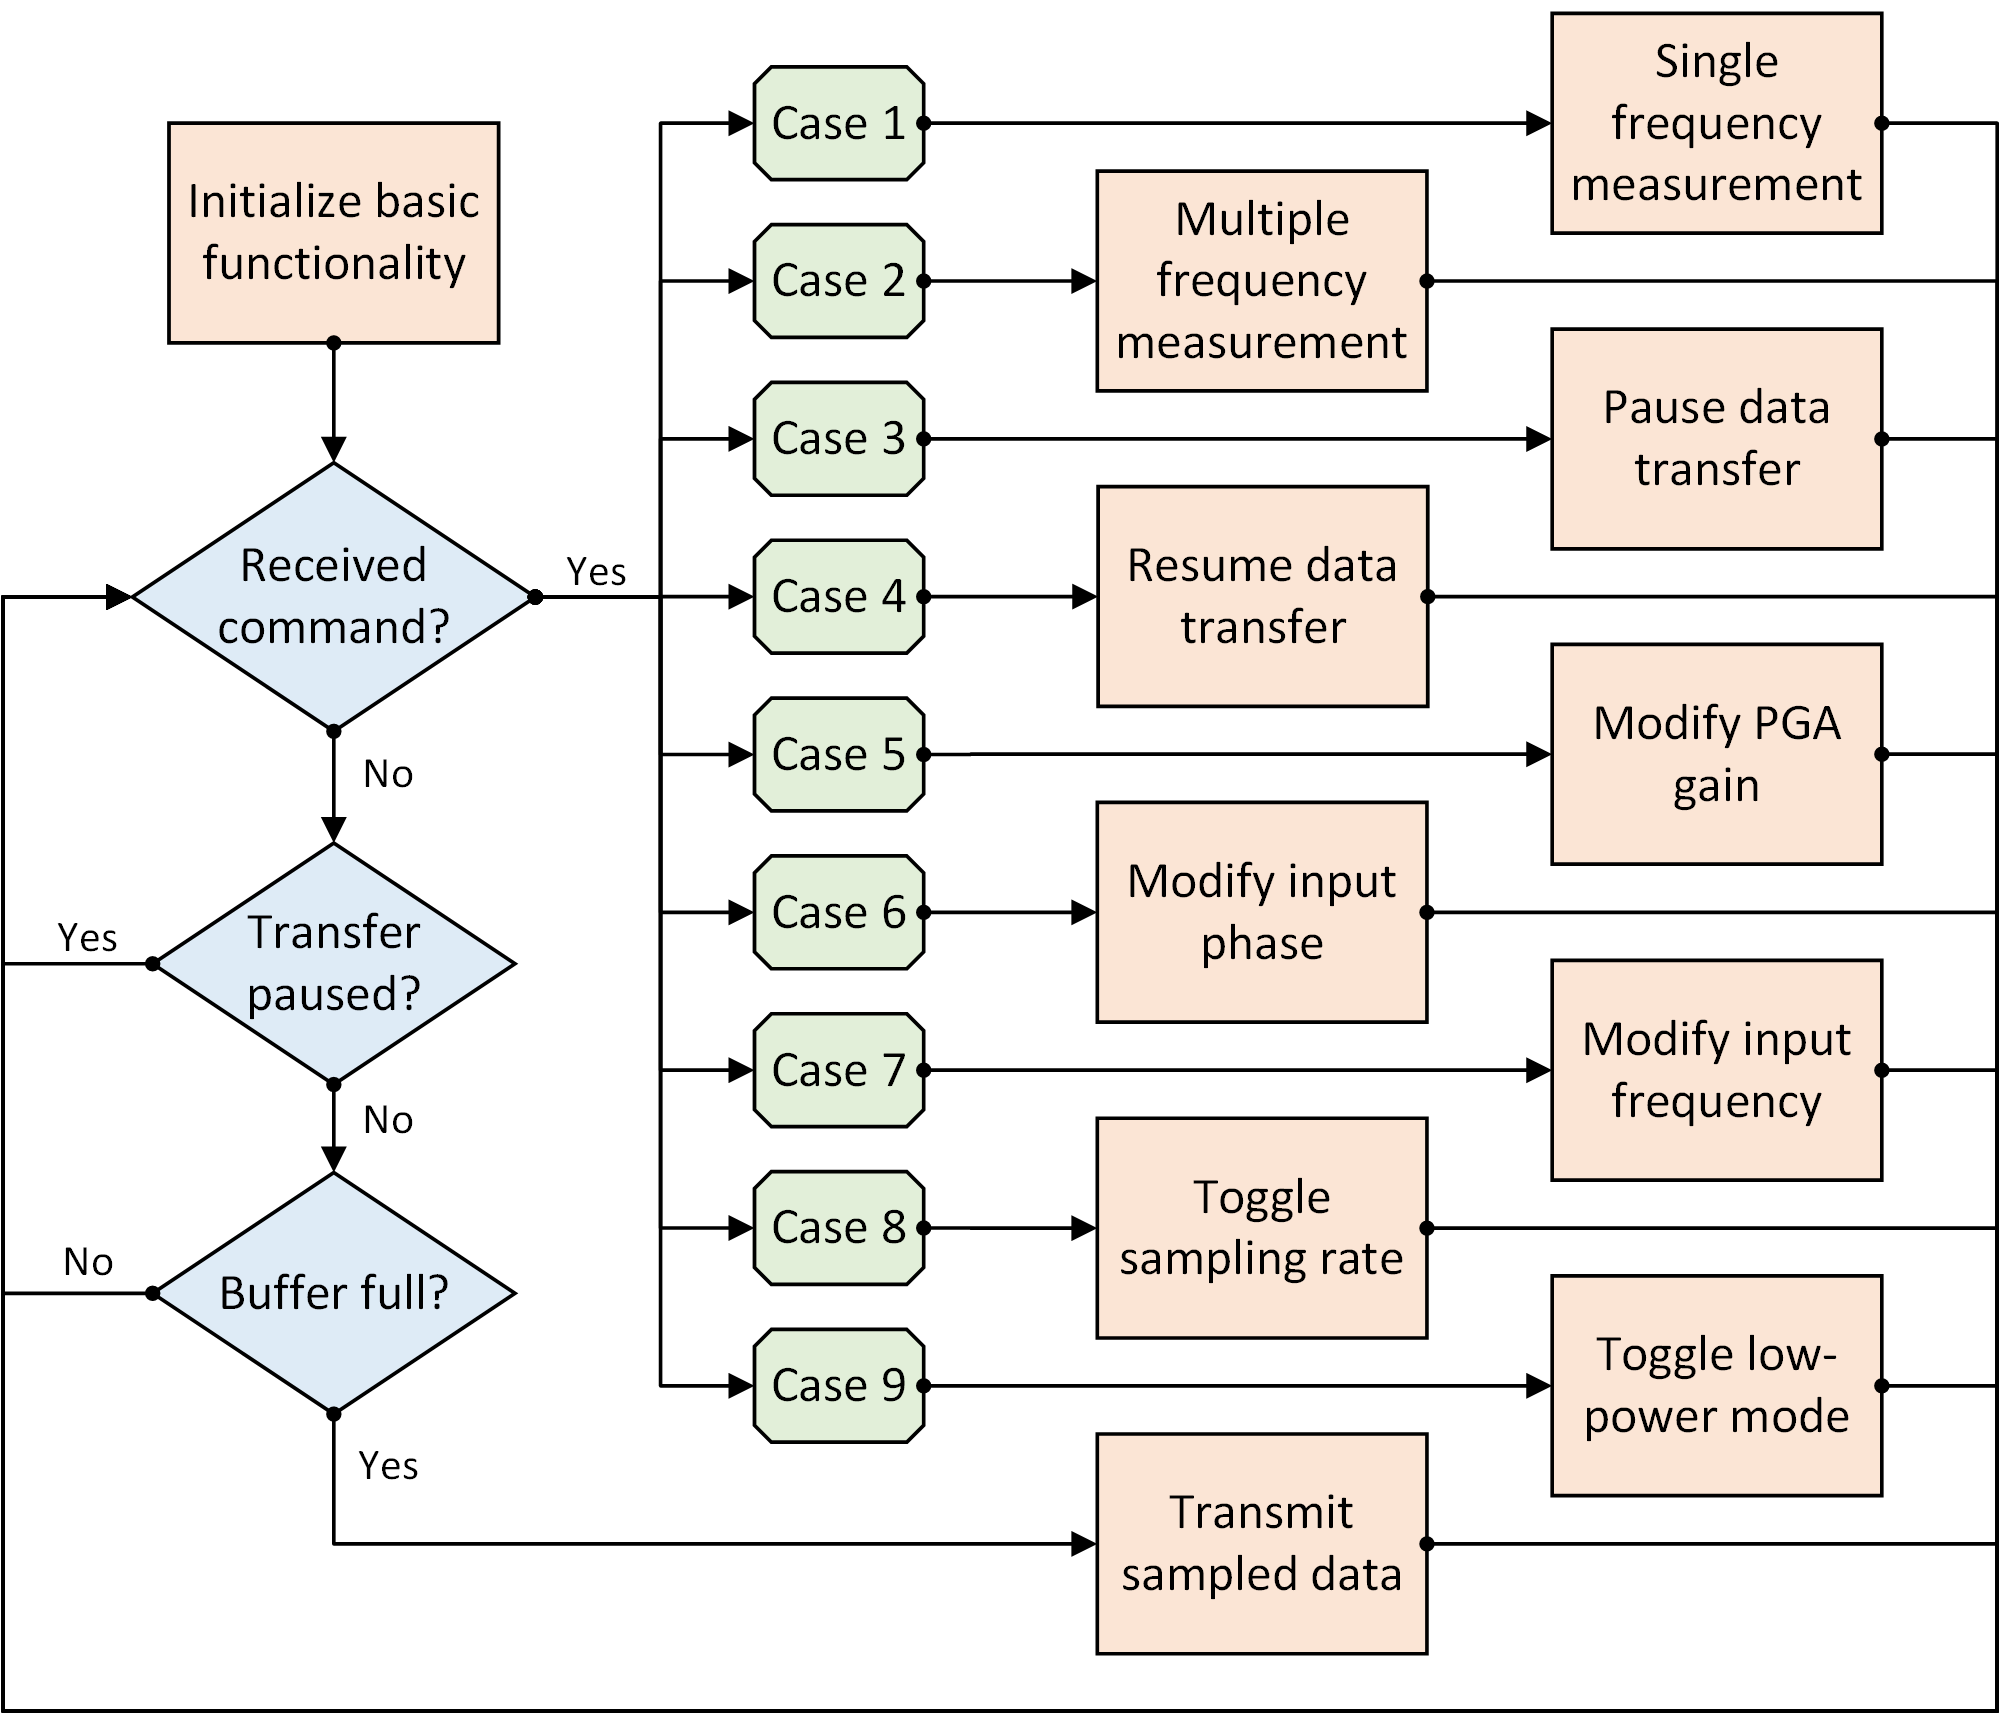
\includegraphics[width=0.95\textwidth]{LoopFlowchart}
    \caption{Flowchart of the MCU for the impedance-sensing system.}
    \label{fig:LoopFlowchart}
\end{figure}

The variable rate sampling works by sampling the data at a high frequency, and only putting the data in the sampling buffer if a significant difference is observed from the few previous samples. This technique is useful in IFC since only the half-sine waveform observed when a particle passes in the channel are useful for the detection. The impedance measured when no particles are in the channel is flat, and only serve to saturate the buffers, which limits the maximum sampling rate of the MCU. As an example, using a variable sampling rate to samples 64 consecutive data points only when a significant difference in measured data is observed increases the maximum practical sampling rate from 655Hz to 5461Hz. %The flowchart of the behaviors of the MCU during the interruptions is given in \autoref{fig:InterruptFlowchart}. \par

%\begin{figure}[h]
%    \centering
%    \includegraphics[width=0.8\textwidth]{InterruptFlowchart}
%    \caption{Flowchart of the interrupt of the MCU for the impedance-sensing system.}
%    \label{fig:InterruptFlowchart}
%\end{figure}

